% %%%%%%%%%%%%%%%%%%%%%%%%%%%%%%%%%%%%%%%%%%%%%%%%%%%%%%%%%%%%%%%%% SECTION FIVE
% %%%%%%%%%%%%%%%%%%%%%%%%%%%%%%%%%%%%%%%%%%%%%%%%%%%%%%%%%%%%%%%%%%%%%%%%%%%%%%
\section{Mid-Side}
Harvey Fletcher, fisico americano, nel 1934 firma uno degli articoli che
compongono un testo cardine per la storia della tecnologia sonora
“\emph{Symposium on Auditory Perspective}”, sulla percezione e la trasmissione
della musica dal vivo, che inizia con le seguenti parole:

\begin{quote}
In this electrical era one is not surprised to hear that orchestral music can be
picked up in one city, transmitted a long distance, and reproduced in another.
Indeed, most people think such things are commonplace. They are heard every
night on the radio. However, anyone who appreciates good music would not admit
that listening even to the best radio gives the emotional thrill experienced in
the concert hall. \cite{hf34}
\end{quote}

Oggi abbiamo perso ogni scintilla di “quell'era elettrica”, anche quella che ha
suscitato la fiamma di interesse nell'ascolto della musica orchestrale
attraverso la trasmissione.

%, o quella che ha suscitato la fiamma di interesse
% nell'ascolto della musica orchestrale, o quella dell'interesse nell'ascolto o,
% molto più semplicemente, la fiamma dell'di interesse. Cento anni dopo quella
% “era” siamo scimmie. Dobbiamo considerare questo fallimento. Inadempienza. Dobbiamo considerare che
% un libro, anche il più inadeguato, in quanto oggetto di pensiero ha potere, come
% dimostrato nell'introduzione, che potrebbe essere il potere di distruggere.

Nel 1964, Paul W. Klipsch introdusse la ristampa del “\emph{Symposium}”:

\begin{quote}
The following paper is a reprint of one of the most important papers in the
field of audio. Fundamentals do not change. The laws of physics endure. In
reprinting the Symposium, the fundamentals are restated. \cite{sap1964}
\end{quote}

Il testo di Fletcher \cite{hf34} è datato 1934, un anno dopo l'approvazione
del brevetto Blumlein che descrive il concetto fondamentale di trasmissione e
registrazione del suono Mid-Side. In quell'epoca gli interessi commerciali e
quelli di ascolto erano intrecciati, in una forma \emph{stereo} solida.

Parlando di orecchie e attività cerebrali per determinare la direzione di una
fonte Blumlein ha scritto:

\begin{quote}
…it is fairly well established that the main factor having effect are phase
differences and intensity differences between the sounds reaching the two ears,
the influence with each of these has depending upon the frequency of the sounds
emitted. For low frequency sound waves there is little or non difference in
intensity at the two ears but there is a marked phase difference. For a give
obliquity of sound the phase difference is approximately proportional to
frequency, representing a fixed time delay between sound arriving at the two
ears, by noting which there is a phase difference of $\pi$ radians or more
between sound arriving at the two ears from a source located on the line joining
them: but above such frequency if phase difference were the sole feature relied
upon for directional location there would be ambiguity in the apparent position
of the source. At the stage however the head begins to became effective as a
baffle and causes noticeable intensity difference between the sounds reaching
the two ears, and it is by noting such intensity difference that brain
determines direction of sounds at higher frequencies\footnote{\cite{ab58} - ...è abbastanza
accertato che il fattore principale sia dovuto alle differenze di fase e di
intensità tra i suoni che raggiungono le due orecchie, l'influenza con ognuna di
queste differenze ha a seconda della frequenza dei suoni emessi. Per le onde
sonore a bassa frequenza c'è poca o nessuna differenza di intensità alle due
orecchie ma c'è una marcata differenza di fase. Per dare un'obliquità del suono,
la differenza di fase è approssimativamente proporzionale alla frequenza, che
rappresenta un ritardo fisso tra il suono che arriva alle due orecchie, notando
che c'è una differenza di fase di $\pi$ radianti o più tra il suono che arriva
alle due orecchie da una sorgente situata sulla linea che le unisce: ma al di
sopra di tale frequenza se la differenza di fase fosse l'unica caratteristica
su cui si basava per la posizione direzionale, ci sarebbe ambiguità nella
posizione apparente della sorgente. Tuttavia, nella fase in cui la testa inizia
a diventare efficace come un deflettore e causa una notevole differenza di
intensità tra i suoni che raggiungono le due orecchie, ed è notando tale
differenza di intensità che il cervello determina la direzione dei suoni a
frequenze più alte.}.
\end{quote}

Sulla base della conoscenza dei meccanismi sopra esposti Blumlein ha formulato
la maggior parte dei principi fondamentali impressi nella storia della stereofonia.
L'approccio più semplice descritto permette di ottenere semplici differenze di livello
nella riproduzione dagli altoparlanti, percepite come differenze di livello e di
fase dalle orecchie. Per ottenere questo tipo di segnale sono necessari almeno due microfoni
posizionati tra loro vicinissimi, allineati verticalmente, in modo da non avere alcun ritardo (orizzontale) tra i canali.
Questa configurazione definita \emph{coincidente} è l'ideale per alimentare
gli altoparlanti con differenze pure di ampiezza tra i canali. Una delle tipiche
tecniche di ripresa stereofonica per coppia coincidente prende proprio il nome
da Blumlein: due microfoni bidirezionali, figura-8 quindi a gradiente di pressione,
angolati tra loro di $\pm45$ gradi, in modo da avere un angolo retto tra loro.

Tuttavia, come esposto nel brevetto, i soli microfoni disponibili a Blumlein nei
suoi primi esperimenti erano non-direzionali a pressione. Coppie stereofoniche coincidenti
con microfoni di questo tipo non sono possibili, in quanto il loro allineamento verticale
produrrebbe due segnali identici, che non descriverebbero stereofonia. È necessaria
quindi una distanza tra i due microfoni. Due microfoni non-direzionali distanziati
anche poco tra loro sono in grado di produrre segnali quasi identici in ampiezza
ma diversi in fase. Blumlein quindi si concentra su una strategia per produrre
anche una differenza di ampiezza tra i due microfoni, inserendo un blocco di legno
tra i due microfoni e progettando una matrice elettrica che mettesse in
relazione i due segnali in modo da produrre le giuste differenze di ampiezza
nell'altoparlante. Il prodotto di tale ricerca fu la matrice di somma e differenza
alla base della tecnologia Mid-Side.

\begin{quote}
\ldots a system of sound transmission wherein the sound
is receive by two or more microphones, wherein at low frequencies difference in
the phase of sound pressure at the microphone is reproduced as difference in
volume at the loud speaker. [\ldots] two microphones transmitted over individual
channels are adapted to interact [\ldots] consisting in half of the sum and half
of the difference respectively of the original \cite{ab58}
\end{quote}

\begin{figure*}[b!]
    \centering
    \begin{subfigure}[t]{0.48\textwidth}
        \centering
        \includegraphics[height=6cm]{CAPITOLI/_TIKZ/POLAR/xy90}
        \caption{Coppia stereofonica coincidente di cardioidi angolati di 90 gradi tra loro in entrata alla matrice.}% \\ Eq: $1(x)$}
        \label{pol:xy90ms}
    \end{subfigure}%
    ~
    \begin{subfigure}[t]{0.48\textwidth}
        \centering
        \includegraphics[height=6cm]{CAPITOLI/_TIKZ/POLAR/midside}
        \caption{Le componenti \emph{Mid-Side} in uscita.}% \\ Eq: $0.75(x)+0.25(x\cos\theta)$}
        \label{pol:midsidems}
    \end{subfigure}
    \caption{Rappresentazione polare ideale del transito di una coppia \emph{xy90}
    attraverso la matrice e relativa rappresentazione d'uscita \emph{Mid-Side}.}
    \label{pol:msmatrix}
\end{figure*}

La matrice di Blumlein di somma e differenza tra i segnali è bidirezionale.
Quando il canale sinistro e destro di una coppia stereofonica passa attraverso la
matrice, la somma di entrambi i canali fornisce il segnale \emph{Mid} contenente solo le componenti in fase,
mentre la differenza produce il segnale \emph{Side} laterale contenente solo
componenti non in fase tra loro. Quando sono le componenti \emph{Mid-Side} a transitare
attraverso la matrice, la somma di \emph{Mid} e \emph{Side} fornisce la
correlazione tra fase sinistra e ampiezza, mentre la differenza produce la
correlazione tra fase negativa a ampiezza.

Di seguito il codice \emph{Faust} per la matrice somma e differenza.

%--------------------------------------------
%----------------larghezza massima del codice
\begin{lstlisting}
nsum = 0.5*(_+_);
ndif = 0.5*(_-_);
sdmx = _,_ <: nsum, ndif;
\end{lstlisting}

%%%%%%%%%%%%%%%%%%%%%%%%%%%%%%%%%%%%%%%%%%%%%%%%%%%%%%%%%%%%%%%%%%%% SECTION SIX
%%%%%%%%%%%%%%%%%%%%%%%%%%%%%%%%%%%%%%%%%%%%%%%%%%%%%%%%%%%%%%%%%%%%%%%%%%%%%%%%
\subsection{Mid-Side \emph{mic}}
\label{subsec:msmic}

\begin{figure}[h]
\centering
\includegraphics[width=1\columnwidth]{CAPITOLI/_TIKZ/POLAR/midside}
\caption{Rappresentazione ideale della coppia stereofonica Mid-Side costituita da
da un microfono direzionale cardioide a gradiente di pressione mediante la sua
equazione polare: $cpg = 0.5(x) + 0.5(x\cos\theta)$ (\emph{cardioid pressure
gradient}) e da un microfono bidirezionale a gradiente di
pressione mediante la sua equazione polare: $bpg = x\cos\theta$
(\emph{bidirectional pressure gradient}). Nella tecnica microfonica di registrazione
Mid-Side il microfono cardioide convenzionalmente viene registrato nel primo canale,
mentre il segnale del microfono bidirezinale viene registrato nel secondo canale.}
\label{polar:midsidemic}
\end{figure}

%%%%%%%%%%%%%%%%%%%%%%%%%%%%%%%%%%%%%%%%%%%%%%%%%%%%%%%%%%%%%%%%%%%% SECTION SIX
%%%%%%%%%%%%%%%%%%%%%%%%%%%%%%%%%%%%%%%%%%%%%%%%%%%%%%%%%%%%%%%%%%%%%%%%%%%%%%%%
\subsection{Mid-Side \emph{panner}}
\label{subsec:mspanner}

Dalla descrizione di Blumlein di \emph{Mid-Side}, abbiamo un canale frontale
\emph{Mid} comunemente descritto da un microfono cardioide.

Infine, il componente Mid del \emph{panner} Mid-Side potrebbe essere espresso dalla
formula

\begin{equation}
m(x,p,\theta) = (p*x) + ((1-p)*(x\cos\theta)
\label{eq:mid}
\end{equation}

Dove $ x $ è il segnale di ingresso, $ p $ è il coefficiente di ampiezza, $0.5$
per scopi cardioidi, $\theta$ è la direzione di impatto angolare espressa in
radianti.

Il componente Side è la formula dritta bipolare di figura 8 che punta a sinistra.

\begin{equation}
s(x,\theta) = x*(sin(\theta))
\label{eq:side}
\end{equation}

Il codice Faust per un \emph{panner} Mid-Side è veramente auto-spiegato: le equazioni
diritte per descrivere sia il cardioide che la figura 8 sono i due componenti
al di fuori del panning.

%--------------------------------------------
%----------------larghezza massima del codice
\begin{lstlisting}
mspan(x,p,rad) = m,s
with{
  m = (p*x)+((1-p)*(x*cos(rad)));
  s = x*(sin(-rad));
};
\end{lstlisting}

\begin{figure}[h]
\centering
\includegraphics[width=1\columnwidth]{CAPITOLI/1000/IMG/mspan}
\caption{Mid-Side \emph{panner}. Il grafico mostra la risposta del \emph{panner} ad una
variazione di 360 gradi da sinistra (-180 gradi) a destra (180 gradi). La linea
laterale (rossa) mostra la
bipolarità del segnale correlata alle informazioni angolari. La linea Mid (blu)
ha solo energia positiva in relazione alle informazioni angolari. La trama
mostra l'evidenza del significato zero su entrambi i bordi di -180 e 180 gradi,
dove cardioide e figura 8 sono senza ascolto.}
\label{fig:mspan}
\end{figure}

Dobbiamo passare il \emph{panner} attraverso la matrice della differenza di somma per
ottenere ciò che Blumlein descrive come la differenza di ampiezza nei segnali
degli altoparlanti dalle differenze di fasi.

%--------------------------------------------
%----------------larghezza massima del codice
\begin{lstlisting}
mspan_lr(x,p,rad) = mspan(x,p,rad) : sdmx;
\end{lstlisting}

\subsection{Utilizzi}

Il \emph{panner} Mid-Side qui proposto non è solo un oggetto tecnico, utile o no,
comparabile o no, relativo ad altri tipi di pan. Il \emph{panner} Mid-Side qui proposto
è un oggetto di pensiero. Usiamo la tecnica Mid-Side, per riflettere la stessa
stereofonia; perché riteniamo fortemente che alcune circostanze evidenziate
nelle sezioni precedenti debbano essere affrontate, altre migliorate e molte
altre uccise.

Pensare al panning deve essere fortemente incoraggiato perché è un oggetto
semplice troppo spesso usato senza fare domande. La gente può pensare che la
chiave quadratica sia migliore di quella lineare che solo in virtù della sua
introduzione più recente. Ma se interrompiamo il suo “utilizzo senza mettere in
discussione” e, come musicisti, prendiamo il tempo per analizzare l'uso manuale
dell'uno al posto dell'altro, possiamo sentire una differenza, pratica prima del
suono.

Conoscendoli possiamo analizzare il mercato del mixer e il ruolo del pan nella
musica di cultura di massa. Senza un \ -a \ -lys \ -ing questi problemi pratici,
non è davvero comprensibile il motivo per cui la peggiore tecnica di panning sia
mai la maggior parte dell'hardware implementato.

Il codice per costruire un \emph{panner} di ampiezza quadratica è piuttosto banale.
Il codice più prolisso \ emph {Faust} lo farà in cinque righe. L'eliminazione di
$sqrt$ dalle seguenti formule diventa il \emph{panner} di ampiezza lineare tradizionale
più semplice.

%--------------------------------------------
%----------------larghezza massima del codice
\begin{lstlisting}
lrpanq(x,p) = l,r
with{
  l = sqrt(1-p)*x;
  r = sqrt(p)*x;
};
\end{lstlisting}

Dove $ p $ è il coefficiente angolare espresso dal potenziometro, in un
intervallo tra $ 0 $ la posizione sinistra, $ 0,5 $ la posizione centrale e $1$
la posizione destra.

Sorridendo, potrebbe essere fatto su una riga:

%--------------------------------------------
%----------------larghezza massima del codice
\begin{lstlisting}
lrpanq(p) = _ <: sqrt(1-p)*_, sqrt(p)*_;
\end{lstlisting}

\begin{figure}[t]
\centering
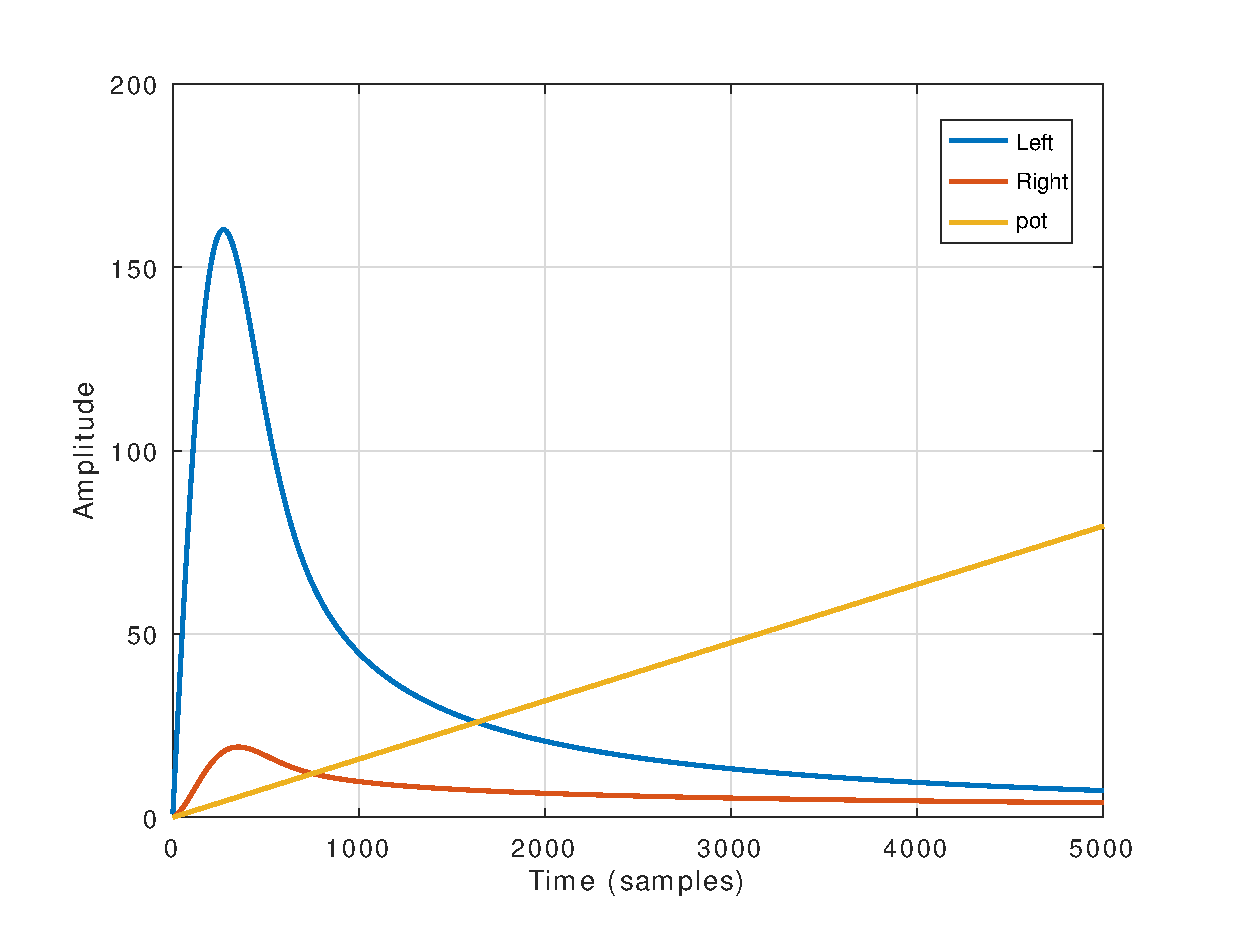
\includegraphics[width=1\columnwidth]{CAPITOLI/1000/IMG/lrpanfb_init}
\caption{\textbf{Risposta feedback \emph{panner} ampiezza quadratica sinistra-destra}.
La trama mostra la risposta del programmatore in un ciclo di scansione da
sinistra a destra. La trama mostra come l'ampiezza si sposta rapidamente oltre
150 volte il valore iniziale sul canale “in feedback” e oltre 20 volte sul
canale “opposto”.}
\label{fig:lrpanfb1}
\end{figure}

\begin{figure}[t]
\centering
\includegraphics[width=1\columnwidth]{CAPITOLI/1000/IMG/lrpanfbpot2}
\caption{\textbf{Risposta feedback \emph{panner} ampiezza quadratica sinistra-destra}.
La trama mostra la risposta del programmatore in un ciclo di scansione da
sinistra a destra. La trama mostra come l'ampiezza si sposta rapidamente oltre
150 volte il valore iniziale sul canale “in feedback” e oltre 20 volte sul
canale “opposto”.}
\label{fig:lrpanfb2}
\end{figure}

Abbiamo spiegato il percorso del pan Mid-Side, partendo dalle radici. Ora è il
momento di capire quali sono i possibili utilizzi e quali sono le peculiarità di
un \emph{panner} Mid-Side invece dei pannolini di ampiezza \emph{tradizionale}.

Il segnale \emph{matrixed} ha la sua complessità come svantaggio. Fermare. In
realtà richiede conoscenza e fantasia per comprendere un segnale come il
significato della combinazione di matrici e richiede anche un po 'di lavoro
complicato più di un segnale diretto.

Come musicisti, anche quando trame e formule appaiono abbastanza chiare, alla
fine, al momento del giudizio, sono le orecchie e l'usabilità musicale a
determinare la scelta migliore, personale.

L'affascinante regno dei segnali \ emph {matrixed} costringe un po 'a lavorare
con il pensiero. Quindi, per noi, ad esempio, la forza di modulazione di fase
del \emph{panner} Mid-Side aveva suggerito, anche prima di un test pratico, una
migliore stabilità sugli utilizzi dal vivo. Perché? È abbastanza semplice da
dimostrare.

Un microfono viene instradato in un canale, con una chiave appuntita a metà
laterale, supponiamo che 23 gradi a sinistra e inviato agli altoparlanti. Con il
panner quadratico, entrambi i canali sinistro e destro hanno valori di ampiezza
diversi con gli stessi valori di fase. Il feedback dei segnali degli
altoparlanti all'interno del microfono proviene da diverse fonti di energia in
fase. La ricerca del feedback con le dita sul guadagno produrrà segnali che
aumenteranno almeno quadraticamente [fig. \ref{fig:lrpanfb1}, \ref{fig:lrpanfb2}].

\begin{figure}[h]
\centering
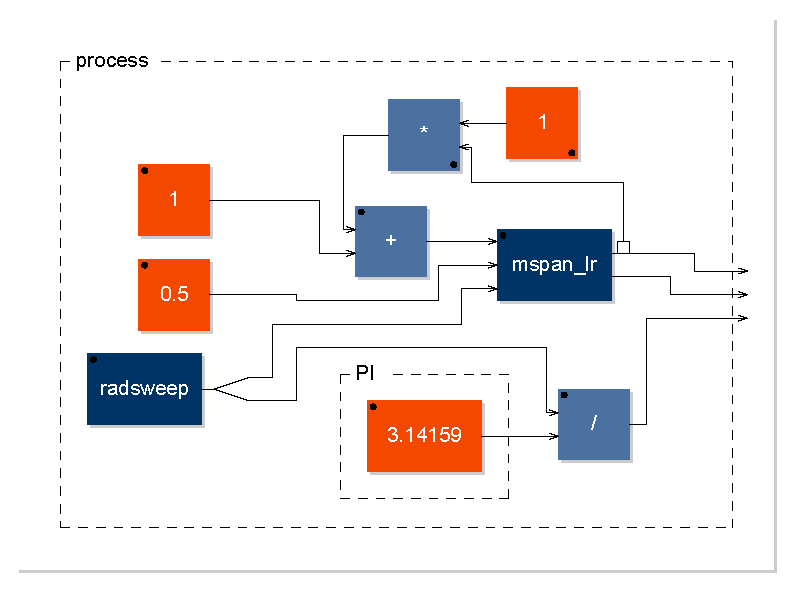
\includegraphics[width=1\columnwidth]{CAPITOLI/1000/IMG/mspanlrfb_diagram}
\caption{\textbf{Block diagram of the infinite feedback}.}
\label{fig:mspanlrfbdiag}
\end{figure}

D'altra parte, nella stessa situazione di feedback, con la stessa provenienza
del panning angolare applicata al segnale del microfono, il pan Mid-Side
produrrà fasi diverse e energia diversa per entrambi gli altoparlanti. Le
differenze, nell'aria, produrranno un modello di feedback più resistivo. In
altre parole, il \emph{panner} di Mid-Side agisce “naturalmente” come anti-\emph{Larsen}.


\begin{figure}[t]
\centering
\includegraphics[width=1\columnwidth]{CAPITOLI/1000/IMG/mspanlrfbpot}
\caption{\textbf{Mid-Side to Left-Right \emph{panner}}. The plot describes the feedback
response with a pan movement through the entire panorama, from -180 to 180
degrees (yellow line, normalized to -1 and 1). The energy multiplies up to four
times for the left channel in infinite feedback (blue line). The top of feedback
increasing is at 45 degrees position in direction of the channel in feedback.}
\label{fig:mspanlrfb}
\end{figure}
